\section{Variace, permutace a kombinace}

Nyní trochu rozšíříme na repertoár nástrojů. Zatím jsme řešili úlohy, kde jsme vybírali vždy "po jednom" prvku, abychom dosáhli jisté konfigurace. Nyní se podíváme, jakých výsledků dosáhneme v případě, kdy budeme již vybírat nějaké $k$-tice z nějaké $n$ prvkové množiny objektů.\par
Je třeba si rozmyslet dva základní případy:
\begin{itemize}
    \item výběr $k$-tic, kde \textbf{záleží na pořadí},
    \item výběr $k$-tic, kde \textbf{nezáleží na pořadí}.
\end{itemize}
S prvním případem jsme již do jisté míry obeznámeni, neboť u úloh, které jsme řešili, vždy záleželo na pořadí. To tedy vede na sestavování tzv. \emph{uspořádaných $k$-tic}, které jsme již zmínili ve formulaci kombinatorického pravidla součinu \ref{thm:pravidlo_soucinu}. Těm říkáme tzv. \textbf{variace $k$-té třídy z $n$ prvků}. Tedy např. variací 2. třídy z množiny $\set{1,\,2,\,3}$ je třeba
\begin{equation*}
    (1,\,3)\;\;\;\text{nebo}\;\;\;(3,\,1).
\end{equation*}

Druhý případ je pro nás novinkou. Vybíráme totiž tzv. \emph{neuspořádané $k$-tice}, tzn. vybereme-li např. z množiny $\set{a,\,b,\,c}$ neuspořádanou dvojici sestávající z prvků $a$ a $c$, pak je to stejné jako výběr neuspořádané dvojice sestávající z prvků $c$ a $a$. Takový výběr nazýváme \textbf{kombinací $k$-té třídy z $n$ prvků}.\par
V rámci tohoto textu se omezíme na tzv. variace, resp. kombinace \textbf{bez opakování}. Výběry s opakováním si zle nastudovat např. ve skriptech \citep[str. 9]{Slavik2022}.
\medskip

Výběrem bez opakování rozumíme výběr $k$-tice prvků takové, že se v ní žádný prvek neopakuje, tzn. každý je v ní nejvýše jednou. Tedy rozlišujeme
\begin{itemize}
    \item \emph{variace bez opakování} a
    \item \emph{kombinace bez opakování}.
\end{itemize}
Pojďme se nyní podívat na metody jejich výpočtu.

\begin{theorem}[Variace bez opakování]\label{thm:variace_bez_opakovani}
    Počet uspořádaných $k$-tic sestavených z $n$-prvkové množiny tak, že se každý prvek ve výběru vyskytne nejvýše jednou, je roven
    \begin{equation*}
        \prod_{i=1}^{k}(n-i+1)=n(n-1)(n-2)\cdots(n-k+1).
    \end{equation*}
\end{theorem}
\begin{proof}
    Tento fakt přímo plyne z kombinatorického pravidla součinu. Na první pozici máme $n$ možností výběru, na druhé $n-1$ možností, \dots a pro $k$-tý člen máme $n-k+1$ možností. Tedy celkově $n(n-1)\cdots(n-k+1)$ možností.
\end{proof}

Počet variací $k$-té třídy z $n$-prvkové množiny bez opakování budeme značit $V_k(n)$.

\begin{task}
    Ve třídě, kde je celkem 25 dětí, si žáci volí nového pokladníka, šatnáře a službu na tabuli, přičemž jeden žák nesmí zastávat více pozic zároveň. Kolika různými způsoby si může třída zvolit žáky na dané pozice.
\end{task}
\begin{solution}
    V tomto případě jistě záleží na pořadí výběru (vybrat žáka na pozici šatnáře není jistě to samé, jako jej vybrat na pozici pokladníka). Tedy budeme počítat variace 3. třídy z 25 prvků bez opakování, tedy existuje
    \begin{equation*}
        V_3(25)\stackrel{\ref{thm:variace_bez_opakovani}}{=}25\cdot(25-1)\cdot(25-2)=25\cdot 24\cdot 23=13\,800\;\text{způsobů.}
    \end{equation*}
\end{solution}

Dalším důležitým, a zatím nezmíněným termínem, je tzv. \emph{permutace}. Permutací rozumíme libovolné uspořádání $n$ prvků do řady. Tedy např. 5, 3, 2, 4, 1 je permutace množiny $\set{1,\,2,\,3,\,4,\,5}$. Permutace lze interpretovat jako uspořádané $n$-tice, což z nich dělá speciální případ variace (výběr uspořádané $n$-tice z $n$ prvkové množiny). Stejně jako u variací a kombinací rozlišujeme permutace s opakováním a bez opakování.
\begin{theorem}[Permutace bez opakování]
    Počet uspořádaných $n$-tic z $n$-prvkové množiny tak, že se každý prvek ve výběru vyskytne nejvýše jednou, je
    \begin{equation*}
        \prod_{i=1}^{n}i=n(n-1)(n-2)\dots 2\cdot 1.
    \end{equation*}
\end{theorem}
\begin{proof}
    Permutace je speciálním případem variace pro $k=n$, tedy $V_n(n)\stackrel{\ref{thm:variace_bez_opakovani}}{=}n(n-1)(n-2)\cdots 2\cdot 1$.
\end{proof}

\begin{definition}[Faktoriál]\label{def:faktorial}
    Je-li $n\in\N_0$, pak definujeme číslo
    \begin{equation*}
        n!=n(n-1)(n-2)\cdots 2\cdot 1=\prod_{i=1}^{n}i,
    \end{equation*}
    které nazýváme \emph{faktoriál} (čteme "$n$ faktoriál"). Speciálně pro $n=0$ definujeme $0!=1$.
\end{definition}

Číslo $n!$ tedy vyjadřuje počet permutací $n$ prvkové množiny\footnote{Podobně jako pro variace, i pro permutaci $n$ prvkové množiny se zřídka používá značení $P(n)$. Avšak je tomu tak málokdy, neboť často se při výpočtech píše rovnou $n!$.}. Zároveň se podívejme ještě na speciální případ $n=0$. Podle naší definice a významu, který přidružujeme faktoriálu, říkáme, že 0 prvků lze seřadit jedním způsobem. (Zkuste si promyslet.)

\begin{task}
    Z 10 knih je 6 psáno česky a zbylé 4 latinsky. Kolika různými způsoby lze daná knihy umístit na poličku, jestliže všechny knihy psané česky mají být vedle sebe a všechny latinsky psané vedle sebe? (Úloha i řešení \cite{Havrlant2022}.)
\end{task}
\begin{solution}
    Všechny české knihy chceme seřadit vedle sebe, tj. jedná se o permutaci na šesti prvcích, kterých je $6!$. Podobně latinsky psané knihy lze vedle sebe seřadit $4!$ způsoby. Seřazení český a latinských knih jsou na sobě nezávislá a tedy podle kombinatorického pravidla součinu existuje
    \begin{equation*}
        6!\cdot 4!=(6\cdot 5\cdot 4\cdot 3\cdot 2\cdot 1)\cdot(4\cdot 3\cdot 2\cdot 1)=720\cdot 24=17\,280\;\text{možností.}
    \end{equation*}
\end{solution}

Zatím jsme se zabývali uspořádanými $k$-ticemi (variace a permutace), jejichž důležitou vlastností bylo, že záleželo na pořadí. Pokud ovšem chceme od pořadí upustit a soustředit se jen na vybrané prvky, budeme muset náš výpočet lehce upravit.

\begin{theorem}[Kombinace bez opakování]\label{thm:kombinace_bez_opakovani}
    Počet neuspořádaných $k$-tic sestavených z prvků $n$ prvkové množiny tak, že se každý prvek ve výběru vyskytne nejvýše jednou, je roven
    \begin{equation*}
        \dfrac{n(n-1)(n-2)\cdots(n-k+1)}{k!}=\dfrac{1}{k!}\prod_{i=1}^{k}(n-i+1)
    \end{equation*}
\end{theorem}
\begin{proof}
    Naši úvahu můžeme založit na následujícím pozorování: máme-li nějakou \emph{neuspořádanou} $k$-tici prvků z $n$ prvkové množiny, pak existuje přesně $k!$ způsobů, jak vybrané prvky uspořádat do řady, čímž z ní vytvoříme \emph{uspořádanou} $k$-tici. To znamená, že platí
    \begin{equation*}
        (\text{počet uspořádaných $k$-tic})=k!\cdot(\text{počet neuspořádaných $k$-tic}).
    \end{equation*}
    Počet neuspořádaných $k$-tic umíme vypočítat podle věty \ref{thm:variace_bez_opakovani}, tedy máme
    \begin{equation*}
        \prod_{i=1}^{k}(n-i+1)=k!\cdot(\text{počet neuspořádaných $k$-tic}).
    \end{equation*}
    Vydělíme-li rovnost číslem $k!$, dostaneme požadovaný výraz, tj.
    \begin{equation*}
        (\text{počet neuspořádaných $k$-tic})=\dfrac{1}{k!}\prod_{i=1}^{k}(n-i+1)
    \end{equation*}
\end{proof}

\begin{definition}[Kombinační číslo]\label{def:kombinacni_cislo}
    Mějme čísla $n,\,k\in\N$. Pak definujeme číslo
    \[
        \binom{n}{k}=\dfrac{n(n-1)(n-2)\cdots(n-k+1)}{k!}=\dfrac{1}{k!}\prod_{i=1}^{k}(n-i+1),
    \]
    které nazýváme \emph{kombinační číslo} (čteme "$n$ nad $k$").
\end{definition}

\begin{remark}\label{rem:kombinacni_cislo_vypocet}
    Kombinační číslo tedy představuje počet možných výběrů neuspořádané $k$-tice z $n$ prvků.\par
    Často se lze však setkat s alternativní definicí
    \[
        \binom{n}{k}=\dfrac{n!}{(n-k)!k!}.
    \]
    Není těžké si rozmyslet, že tento vzorec říká to samé, co vzorec ve větě \ref{thm:kombinace_bez_opakovani}. Avšak zde je třeba si dávat pozor, že vzorec platí pouze, pokud je $k\leqslant n$, protože pro $k>n$ by byl výraz $n-k$ záporný a jeho faktoriál by tak nebyl definován. Avšak ve vzorci
    \[\dfrac{n(n-1)(n-2)\cdots(n-k+1)}{k!}\]
    se pro $k>n$ vyskytne v čitateli zlomku u jednoho z činitelů 0 (neboť se zde vždy vyskytne výraz $n-(n+1)+1$ pro $k=n+1$) a tedy i celý součin bude nulový. To dává ostatně i smysl, neboť neuspořádanou $k$-tici $n$ prvků bez opakování při $k>n$ nelze vybrat žádným způsobem. Nicméně pro $k>n$ je někdy tvar
    \[\dfrac{n!}{(n-k)!k!}\]
    výhodný při výpočtech.
\end{remark}

\begin{task}
    Petr má sedm knih, o které se zajímá Ivana, Ivana má deset knih, o které se zajímá Petr. Určete, kolika způsoby si Petr může vyměnit dvě své knihy za dvě knihy Ivaniny. \citep[sekce \emph{Kombinace}]{Farska2007}
\end{task}
\begin{solution}
    Ivana a Petr každý vybírají 2 knihy, které si vymění s tím druhým. Na pořadí výběru knih nezáleží. Celkově se tedy bude jednat \emph{kombinace 2. třídy ze 10 prvků} a \emph{kombinace 2. třídy ze 7 prvků}. Každý z výběrů je však nezávislý, tedy podle kombinatorického pravidla součinu dostáváme
    \[\binom{10}{2}\binom{7}{2}\stackrel{\ref{rem:kombinacni_cislo_vypocet}}{=}\dfrac{10!}{(10-2)!2!}\cdot\dfrac{7!}{(7-2)!2!}=\dfrac{10\cdot 9\cdot \cancel{8!}}{\cancel{8!}\cdot 2}\cdot\dfrac{7\cdot 6\cdot\cancel{5!}}{\cancel{5!}\cdot 2}=5\cdot 9\cdot 7\cdot 3=945\;\text{možností.}\]
\end{solution}

\begin{task}
    Je dán čtverec ABCD a na každé jeho straně n ($n\geqslant 3$) vnitřních bodů. Určete počet všech trojúhelníků s vrcholy v těchto bodech. \citep[sekce \emph{Kombinace}]{Farska2007}
\end{task}
\begin{figure}[H]
	\centering
	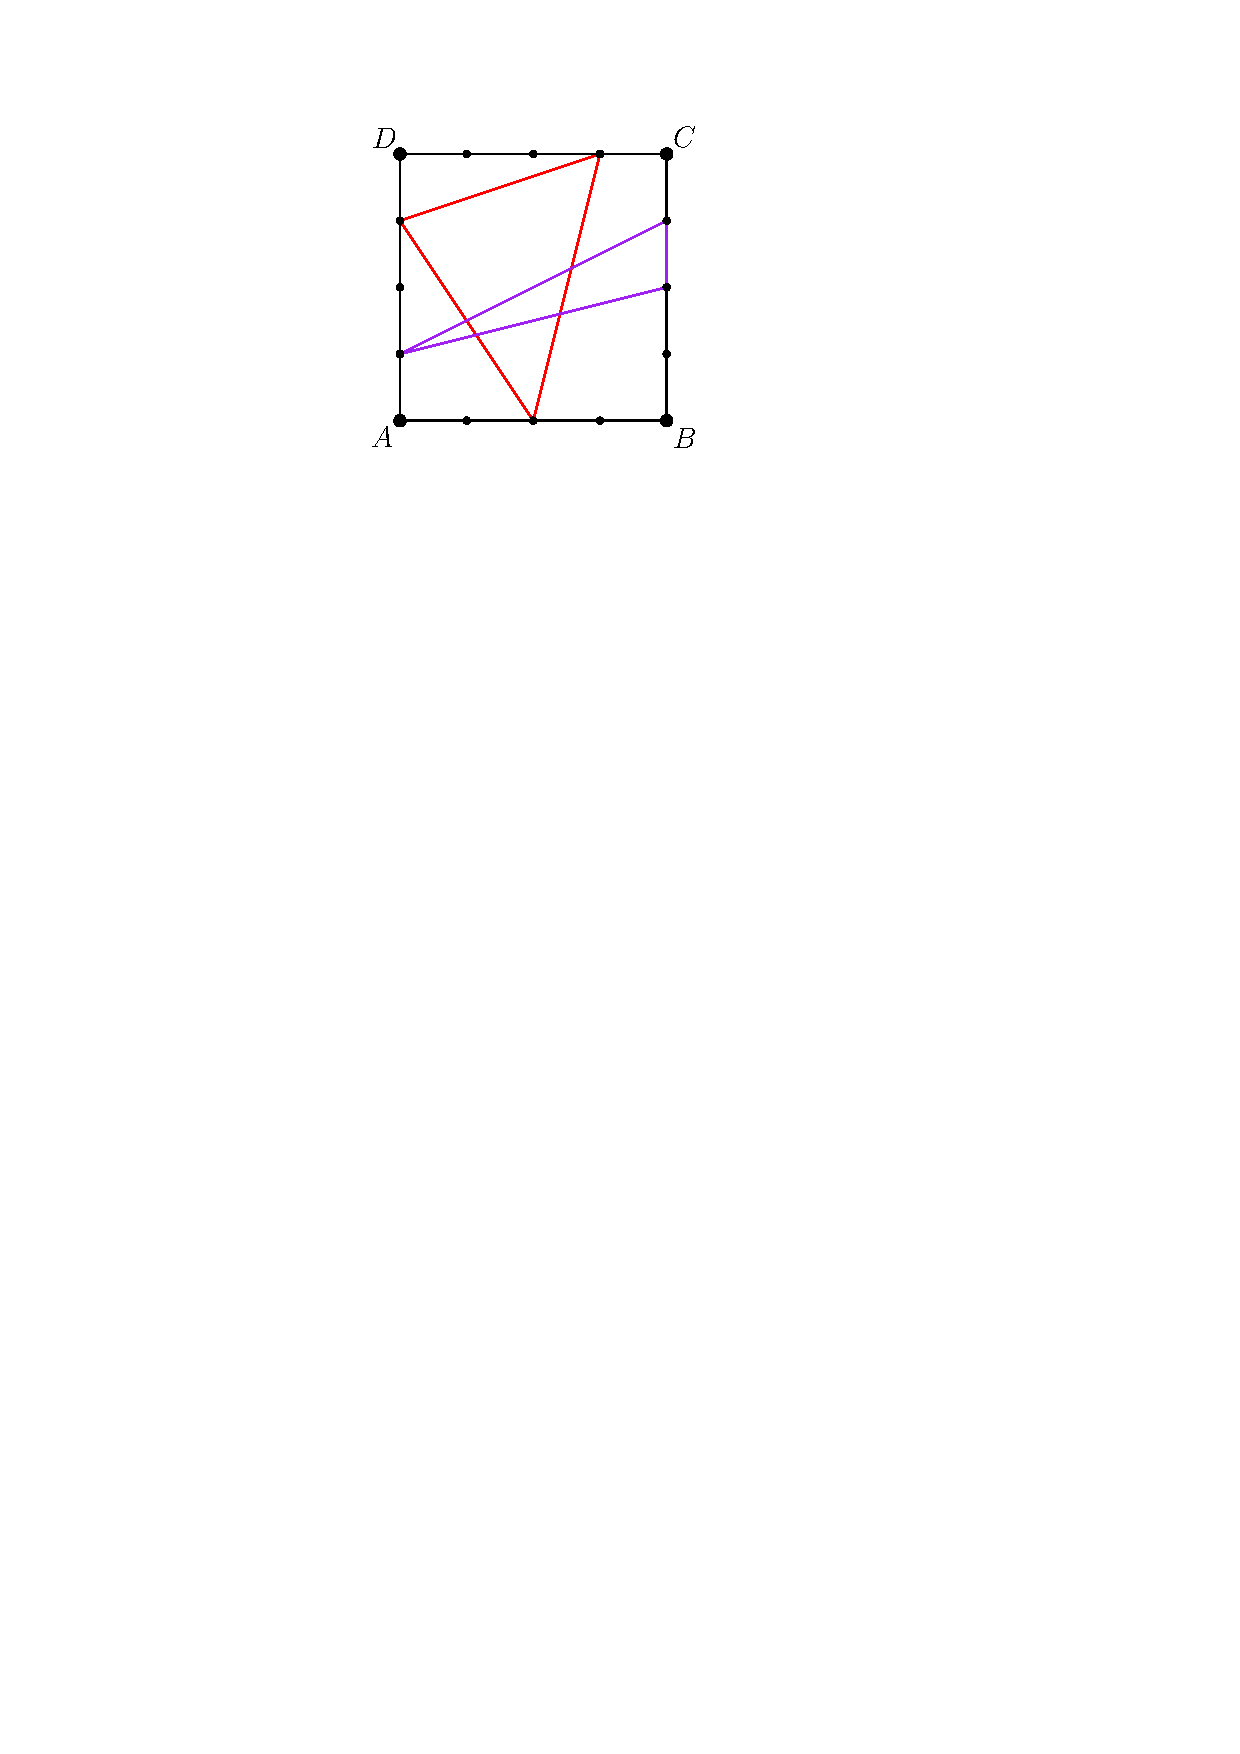
\includegraphics[scale=\normalipe]{ch02_trojuhelnik_ve_ctverci.pdf}
    \caption{Ukázka trojúhelníků ve čtverci ABCD.}
    \label{fig:trojuhelniky_ve_ctverci}
\end{figure}
\begin{solution}
    V tomto případě stačí ze všech dostupných bodů (kterých je $4n$) vybrat všechny možné trojice. Je třeba mít však na paměti, že trojúhelník vznikne pouze volbou bodů, které neleží na jedné přímce, tzn. body nesmí všechny ležet na jedné straně čtverce ABCD. Tyto varianty jsou však započítány ve výrazu $\binom{4n}{3}$, tedy je třeba je odečíst. Na libovolné straně nepřipouštíme žádnou kombinaci tří bodů na ní ležících, těch je $\binom{n}{3}$ a pro všechny strany tedy $4\cdot \binom{n}{3}$. Celkově tedy existuje
    \[\binom{4n}{3}-4\cdot\binom{n}{3}\;\text{různých trojúhelníků.}\]
\end{solution}

\begin{task}
    Určete, kolika způsoby je možno ze dvaceti osob vybrat deset, požadujeme-li, aby mezi vybranými
    \begin{enumerate}[label=(\alph*)]
        \item nebyl pan A;
        \item nebyli zároveň pánové A a B;
        \item byl aspoň jeden z pánů A, B.
    \end{enumerate}
    \citep[sekce \emph{Kombinace}]{Farska2007}
\end{task}
\begin{solution}[Řešení (a)]
    Pokud nechceme, aby mezi vybranými lidmi byl pan A, pak vybíráme všechny kombinace 10. třídy takové, že neobsahují pana A, tj. ze zbývajících devatenácti osob. Takových výběrů existuje
    \[\binom{19}{10}\stackrel{\ref{rem:kombinacni_cislo_vypocet}}{=}\dfrac{19!}{(19-10)!10!}=\dfrac{19\cdot 18\cdots\cancel{10!}}{9!\cdot\cancel{10!}}=92\,378.\]
\end{solution}
\begin{solution}[Řešení (b)]
    Pokud nemají být mezi vybraný lidmi pánové A a B \textbf{zároveň}, pak ovšem připouštíme varianty, kdy je ve vybrané skupině pouze pan A, nebo pouze pan B. K výpočtu lze přistoupit takto:
    \begin{enumerate}[label=(\roman*)]
        \item vypočítáme počet všech skupinek,
        \item odečteme počet skupinek, kde se nachází pan A a pan B zároveň.
    \end{enumerate}
    V případě \textit{(i)} se jednoduše jedná o kombinaci 10. třídy z 20 prvků, tj. $\binom{20}{10}$. V případě \textit{(ii)} lze skupinky, kde se nachází pan A a zároveň pan B, následovně: uvážíme, že pan A a pan B jsou již ve vybrané skupince a nyní k nim přidáme ze zbylých osmnácti lidí osm, tj. $\binom{18}{8}$. Tedy celkově existuje
    \[\binom{20}{10}-\binom{18}{8}=140\,998\]
    výběrů, kde se nenachází pan A a zároveň pan B.
\end{solution}
\begin{solution}[Řešení (c)]
    Zde by nás mohlo napadnou spočítat počet těchto výběrů tak, že sečteme skupinky, kde se nachází pan A a skupinky, kde se nachází pan B. Problém však je, že tím bychom některé možnosti započítali vícekrát (specificky ty, kde se nachází pan A, i pan zároveň). Zkusme proto obdobou strategii, jako v \textit{(b)}. Od celkového počtu možných výběrů libovolné skupinky, který je $\binom{20}{10}$, odečteme ty, kde se nenachází ani pan A, ani pan B. To odpovídá výběru desetičlenné skupinky ze zbylých osmnácti lidí, tj. $\binom{18}{10}$. Celkově tak existuje
    \[\binom{20}{10}-\binom{18}{10}=140\,998\]
    výběrů\footnote{Může se možná zdát zarážející, že výsledek je stejný, jako v bodě \textit{(b)}, nicméně později se dozvíme, proč tomu tak je. Není to náhoda. :-)}, kde se nachází aspoň jeden z panů A, B.
\end{solution}